\section{Reale Bauteile}

\subsection{Impedanzen -- Übersicht}

$$ \boxed{ Z_C = \frac{1}{\jimg \omega C} } 
    \qquad \boxed{ Z_L = \jimg \omega L } 
    \qquad \boxed{ |Z| = \sqrt{R_{\rm tot}^2 + X_{\rm tot}^2 } }
    \qquad \boxed{ f_{\rm res} = \frac{1}{2 \pi \sqrt{ R C} } } $$


\subsection{Reale Widerstände}

\begin{minipage}[c]{0.20\columnwidth}
    $$ \boxed{R = \frac{\rho \cdot l}{A}} $$
\end{minipage}
\hfill
\begin{minipage}[c]{0.78\columnwidth}
    \begin{tabular}{llc}
        $R$     & spez. Widerstand ($@ \, 20 \, \degree$)   & $[R] = \ohm$ \\
        $\rho$  & spez. Widerstand                          & $[\rho] = \frac{\ohm \milli \meter^2}{\meter}$ \\
        $l$     & Länge des Leiters                         & $[l] = \meter$ \\
        $A$     & Querschnitt des Leiters                   & $[A] = \meter^2$
    \end{tabular}
\end{minipage}


\subsubsection{Ersatzschaltung und Frequenzabhängigkeit}

\begin{minipage}[c]{0.48\columnwidth}
    % TODO: Ersatzschaltung in tikz

    \begin{tabular}{ll}
        $R$     & nom. Widerstand  \\
        $L_S$   & Zuleitung \\
        $C$     & zwischen Anschlüssen
    \end{tabular}
\end{minipage}
\hfill
\begin{minipage}[c]{0.5\columnwidth}
    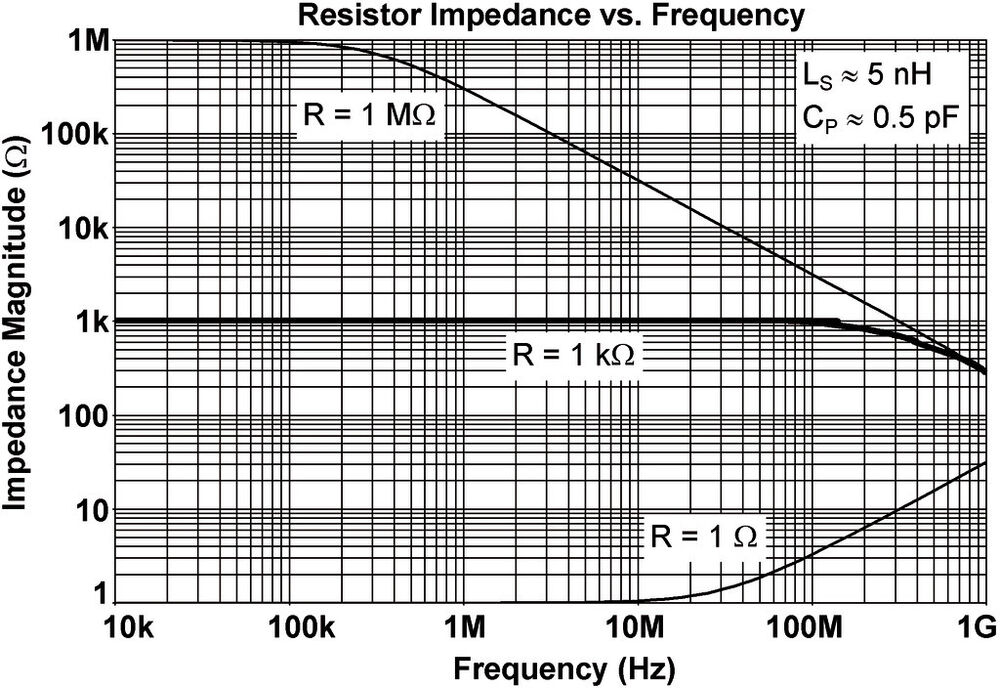
\includegraphics[width=\columnwidth]{images/realer_widerstand_frequenzverlauf.jpg}

    \begin{tabular}{ll}
        Grosse Widerstände  & \textrightarrow\ R und C \\
        Kleine Widerstände  & \textrightarrow\ R und L \\
    \end{tabular}
\end{minipage}


\subsubsection{Temperaturabhängigkeit}

%copy-paste vom Anhang
\begin{minipage}[c]{0.3\columnwidth}
    $$ \boxed{R_{\vartheta} = R_{20} + \Delta R} $$
    $$ \boxed{\Delta R = R_{20} \cdot \alpha \cdot \Delta \vartheta} $$
\end{minipage}
\hfill
\begin{minipage}[c]{0.68\columnwidth}
    \begin{tabular}{c l c}
        $R_{\vartheta}$     & Widerstand bei Temperatur $\vartheta$             & $[R_{\vartheta}] = \ohm$ \\
        $R_{20}$            & Widerstand bei $20 \, \celsius$                   & $[R_{20}] = \ohm$ \\
        $\alpha$            & Temperaturkoeffizient                             & $[\alpha] = \frac{1}{\kelvin}$\\
        $\Delta \vartheta$  & Temperaturdifferenz $\vartheta - 20 \, \celsius$  & $[\Delta \vartheta] = \celsius$\\
    \end{tabular}
\end{minipage}

\vspace{0.2cm}
\textbf{Achtung:} Leistungs-Derating bei steigender Temperatur beachten!


\begin{minipage}[t]{0.48\columnwidth}
    \subsubsection{Kenngrössen}

    \begin{itemize}
        \item Widestandswert
        \item Toleranz
        \item Temperaturkoeffizient $\alpha$
        \item max. Verlustleistung
    \end{itemize}
\end{minipage}
\hfill
\begin{minipage}[t]{0.48\columnwidth}
    \subsubsection{Auswahlkriterien}
    
    \begin{itemize}
        \item Bauform (Grösse)
        \item Leistung (Verlustwärme)
        \item Widerstandsmaterial
        \item Genauigkeit und Langlebigkeit
    \end{itemize}
\end{minipage}


\subsection{Spezielle Widerstände}

\subsubsection{Thermistoren}

Thermistoren sind \textbf{temperaturabhängige} Widerstände.


\begin{minipage}[c]{0.48\columnwidth}
    \myul{\textbf{NTC (neg. temp. Koeffizient, Heissleiter)}}
\end{minipage}
\hfill
\begin{minipage}[c]{0.48\columnwidth}
    \myul{\textbf{PTC (pos. temp. Koeffizient, Kaltleiter)}}
\end{minipage}


\subsubsection{Varistoren}

Varistoren sind \textbf{spannungsabhängige} Widerstände.


\subsubsection{Fotowiderstände (LDR)}






\subsection{Reale Kondensatoren}

\begin{minipage}[c]{0.20\columnwidth}
    $$ \boxed{C = \frac{\varepsilon_0 \cdot \varepsilon_r \cdot A}{d}} $$
\end{minipage}
\hfill
\begin{minipage}[c]{0.78\columnwidth}
    \begin{tabular}{llc}
        $C$             & Kapazität (\textbf{Plattenkondensator!})          & $[C] = \farad$ \\
        $\varepsilon_0$ & eleltrische Feldkonstante $8.85 \cdot 10^{-12}$   & $[\varepsilon_0] = \frac{\farad}{\meter}$ \\
        $\varepsilon_r$ & relative Permittivität                            & $[\varepsilon_r] = 1$ \\
        $A$             & Fläche der Platten                                & $[A] = \meter$ \\
        $d$             & Abstand zwischen Platten                          & $[d] = \meter$

    \end{tabular}
\end{minipage}


\subsubsection{Ersatzschaltung und Frequenzabhängigkeit}

\begin{minipage}[c]{0.48\columnwidth}
    % TODO: Ersatzschaltung in tikz

    \begin{tabular}{ll@{}}
        $C$             & nom. Kapazität  \\
        $R_{\rm leak}$  & Leckströme (vernachlässigbar!) \\
        $\rm{ESR}$      & Anschlüsse, Zuleitung \\ 
        $\rm{ESL}$      & Anschlüsse, Zuleitung 
    \end{tabular}
\end{minipage}
\hfill
\begin{minipage}[c]{0.5\columnwidth}
    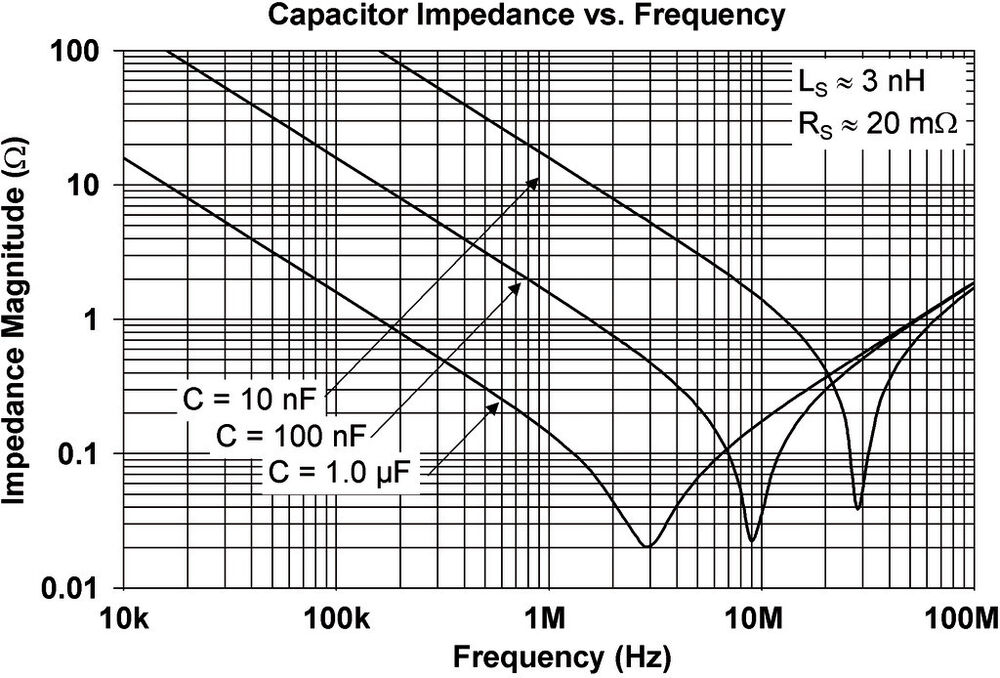
\includegraphics[width=\columnwidth]{images/realer_kondensator_frequenzverlauf.jpg}
\end{minipage}

\begin{minipage}[c]{0.48\columnwidth}
    $$ \boxed{ |Z| = \sqrt{|R|^2 + (|X_{C}| - |X_L|)^2 } } $$
\end{minipage}
\hfill
\begin{minipage}[c]{0.48\columnwidth}
    Bei Resonanz: $ |X_C| = |X_L|$ \textrightarrow\ $Z$ rein resistiv (tiefster Punkt in Diagramm)
\end{minipage}


\subsubsection{Temperaturabhängigkeit}


\subsubsection{Spannungsabhängigkeit}



\subsubsection{Verschiedene Typen von Kondensatoren}

% TODO
\begin{outline}
    \1 \textbf{Elektrolytkondensatoren (Elkos)}
        \2 bla
    \1 \textbf{Tantalkondensatoren}
        \2 bla
    \1 \textbf{Folien-Filmkondensatoren}
        \2 Sind selbstheilend 
        \2 Hohe Genauigkeit
        \2 Relativ teuer
    \1 \textbf{Kondensatoren mit einstellbarer Kapazität}
        \2 Zum Einstellen von Schwingfrequenzen
        \2 Trimmer
    \1 \textbf{Super-Caps}
        \2 Kapazitäten bis $3000 \, \farad$
        \2 $10 \, \%$ Energiedichte von Akkus
        \2 10-fache Leistungsdichte von Akkus
        \2 Können schnell geladen / entladen werden
        \2 Sehr kleine Spannungsfestigkeit
\end{outline}


\subsection{Reale Spulen}

% TODO
\begin{minipage}[c]{0.20\columnwidth}
    
    $$ \boxed{R = \frac{\rho \cdot l}{A}} $$
\end{minipage}
\hfill
\begin{minipage}[c]{0.78\columnwidth}
    \begin{tabular}{llc}
        $R$     & spez. Widerstand ($@ \, 20 \, \degree$)   & $[R] = \ohm$ \\
        $\rho$  & spez. Widerstand                          & $[\rho] = \frac{\ohm \milli \meter^2}{\meter}$ \\
        $l$     & Länge des Leiters                         & $[l] = \meter$ \\
        $A$     & Querschnitt des Leiters                   & $[A] = \meter^2$
    \end{tabular}
\end{minipage}


\subsubsection{Ersatzschaltung und Frequenzabhängigkeit}

\begin{minipage}[c]{0.58\columnwidth}
    % TODO: Ersatzschaltung in tikz

    \begin{tabular}{ll}
        $R$     & nom. Widerstand  \\
        $L_S$   & Zuleitung \\
        $C$     & zwischen Anschlüssen
    \end{tabular}
\end{minipage}
\hfill
\begin{minipage}[c]{0.4\columnwidth}
    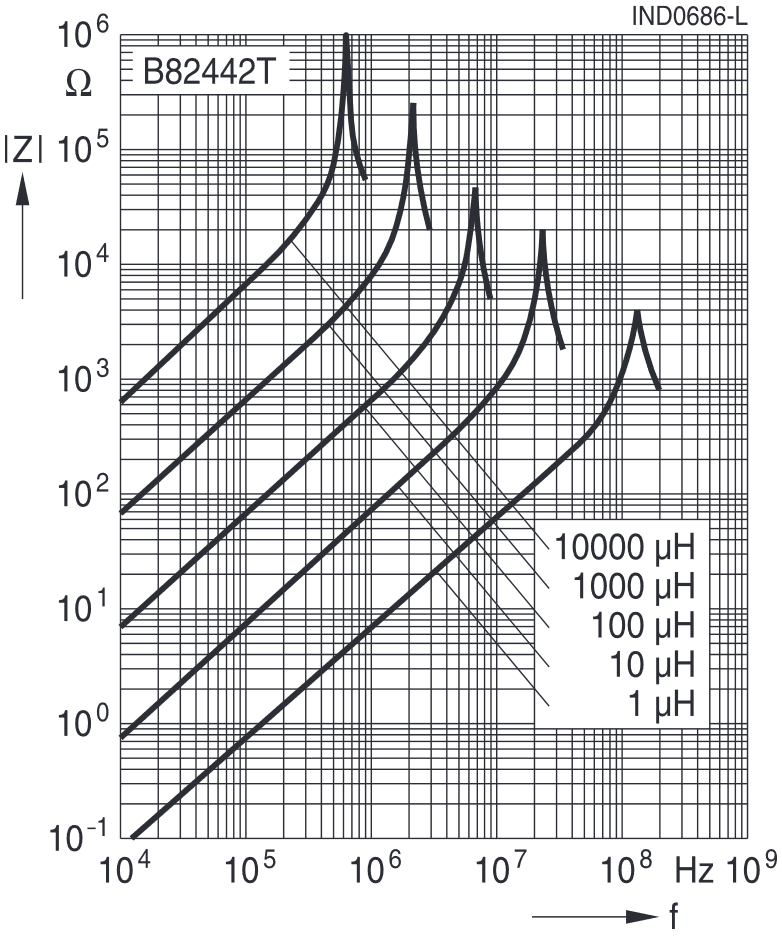
\includegraphics[width=\columnwidth]{images/reale_spule_frequenzverlauf.png}

\end{minipage}